%%%%%%%%%%%%%%%%%%%%%%%%%%%%%%%%%%%%%%%%%%%%%%%%%%%%%%%%%%%%%%%%%%%%
\section{Slow Controls}
\label{sec:fdgen-slow-cryo-ctrl}

% same for SP and DP

The slow controls system will collect, archive, and display data from
a broad variety of sources, and will provide real time alarms and
warnings for detector operators. Data is acquired via network
interfaces.  Figure \ref{fig:gen-slow-controls-diagram} shows the
connections between major parts of the slow controls system and other
systems.  The following subsections describe the required hardware and
software for the slow controls.

\begin{dunefigure}[Slow Controls connections and data]{fig:gen-slow-controls-diagram}
{Typical Slow Controls system connections and data flow}
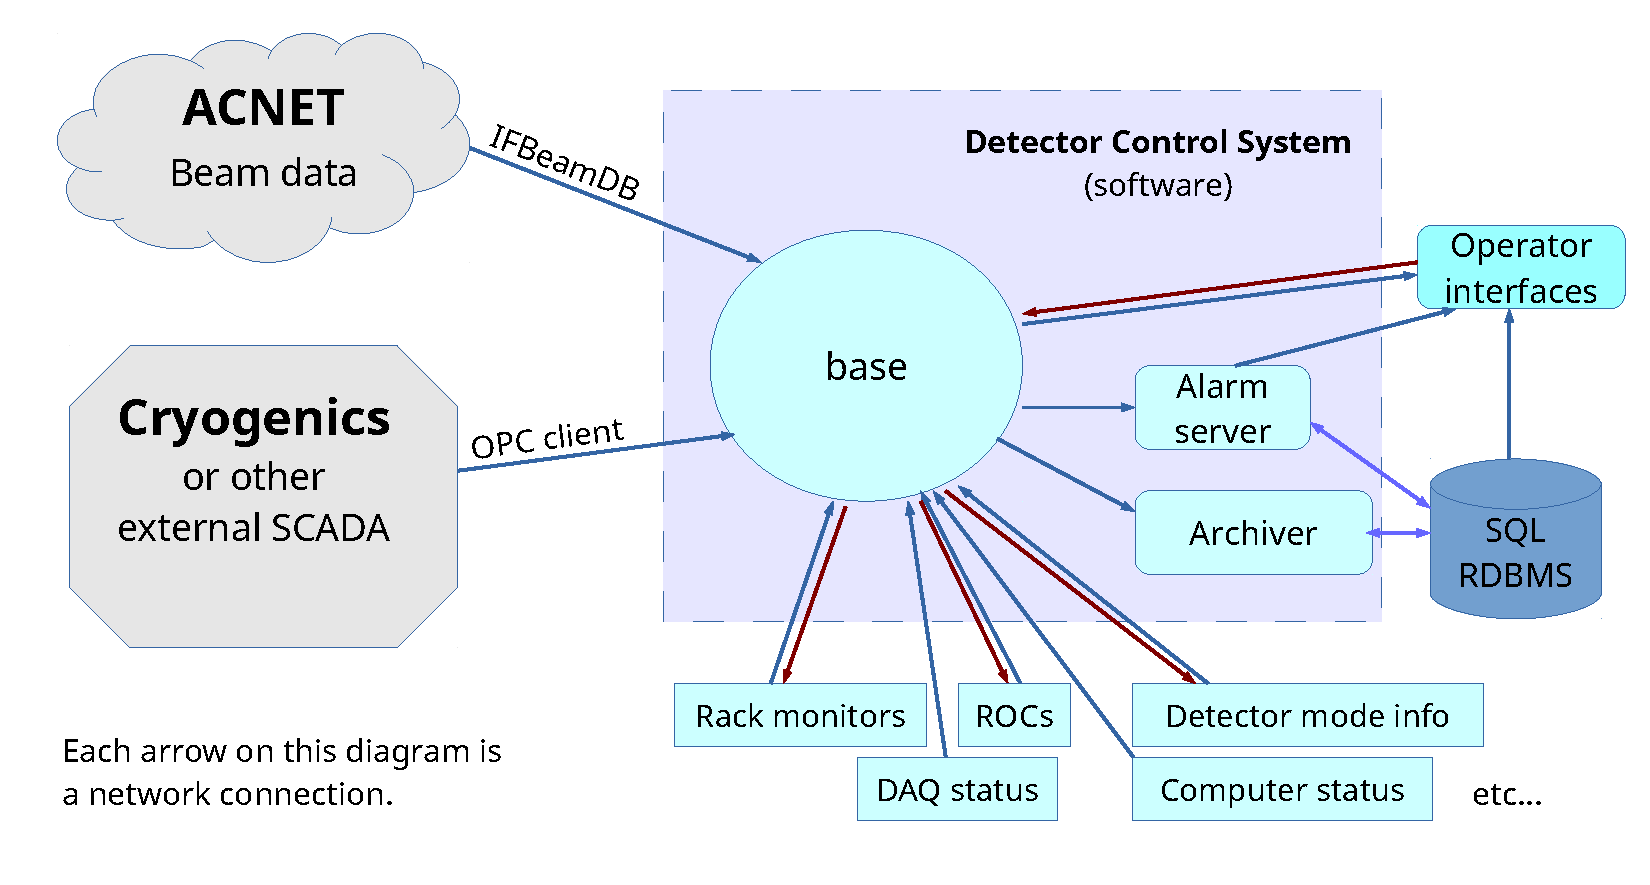
\includegraphics[width=0.7\textwidth]{slow-controls-diagram}
\end{dunefigure}





%%%%%%%%%%%%%%%%%%%%%%%%%%%%%%%%%%%
\subsection{Slow Controls Hardware}
\label{sec:fdgen-slow-cryo-hdwr}

% % % % Alec
\subsubsection{Slow Controls Network Hardware}
\label{sec:fdgen-slow-cryo-slow-network}
The Slow Controls data originates from the sensors discussed in
Sec.~\ref{sec:fdgen-cryo-instr}, then heads towards the central
CISC database housed in the CUC DAQ room
(Sec.~\ref{sec:fdgen-slow-cryo-slow-compute}).  It gets there over
conventional network hardware from any sensors located in the cryogenic
plant.  However, the readouts which are located in the racks on top the
cryostats have to be careful about grounding and noise.  Therefore, each
rack on the cryostat will have a small network switch which will send
any network traffic from that rack to the CUC via a fiber transponder.

Network traffic out of SURF to Fermilab will be primarily database calls
to that central CISC DB: either from monitoring applications, or from
database replication to the offline version of the CISC DB.  This
traffic is of a low enough bandwidth that the proposed general purpose
links both out of the mine and back to Fermilab can accommodate it.

% % % % Alec
\subsubsection{Slow Controls Computing Hardware}
\label{sec:fdgen-slow-cryo-slow-compute}

Up to two racks of space and appropriate power and cooling are available
in the CUC's DAQ server room for CISC usage.  Somewhat less space than
that is currently envisioned: Two servers (a primary server and a
replicated backup) suitable for the needed relational database discussed
in Sec.~\ref{sec:fdgen-slow-cryo-sw} will be there, with an additional
two servers to perform front-end monitoring interface services: for
example, assembling dynamic CISC monitoring web pages from the adjacent
databases.  Any special purpose software, such as iFix or EPICS, would
also run here: two more servers (for a total of six) will accommodate
these programs.\fixme{I am completely making up how many special purpose
  iFix machines there should be: need input from the cryo people}
Replicating this setup on a per-module basis would allow for easier
commissioning and independent operation, accommodate different module
design (and the resulting differences in database tables), and ensure
sufficient capacity.  Including fours sets of networking hardware, this
would fit tightly into one rack or very comfortably into two.

% % % % Alec and Sowjanya
%% \subsubsection{Slow Controls Signal Processing Hardware}
%% Dropped because slow controls scope is defined not to include it.
%% (Signal processing should be within the scope of the hardware
%% generating the signal -- and so should digitization, for that matter.)
%%
%% N.B. The ``laundry list of Things to Be Monitored'' is in
%% \ref{sec:fdgen-slow-cryo-quant}



%%%%%%%%%%%%%%%%%%%%%%%%%%%%%%%%%%%
% Alec
\subsection{Slow Controls Infrastructure}
\label{sec:fdgen-slow-cryo-slow-infra}

%%%%%%%%%%%%%%%%%%%%%%%%%%%%%%%%%%
% Sowjanya
\subsection{Slow Controls Software}
\label{sec:fdgen-slow-cryo-sw}

% same for SP and DP

The Slow Controls software will need to include the following components
to provide complete monitoring and control of detector sub-systems:
%
\begin{description}
 \item{Control systems base} that performs input and output operations
  and defines processing logic, scan conditions, alarm conditions,
  archiving rate, etc.;
 \item{Alarm server} that monitors all channels and sends alarm
  messages to operators; 
 \item{Data archiver} that performs automatic sampling and storage of
  values for history tracking;
 \item{Integrated Operator interface} that provides display panels for
  controls and monitoring.
\end{description}

An additional requirement for the software is to be able to indirectly
interface with external systems ({\em e.g.}\ Cryogenics control
system) and databases ({\em e.g.}\ beam database) to export data into
slow controls process variables (or channels) for archiving and status
displays. This allows integrating displays and warnings into one
system for the experiment operators, and to provide integrated
archiving for sampled data in the archived database. In this case, one
can imagine an Input Output Controller (IOC) running on a central DAQ
server provides ``soft'' channels for these data.
Fig.\ \ref{fig:gen-slow-controls-diagram} shows a typical workflow of a
slow controls system.

In terms of key features of the software, a highly evolved software is
needed that is designed for managing real-time data exchange, scalable
to large number of channels and high bandwidth if needed. The software
should be well documented, supported, and known to be reliable. The base
software should also allow easy access of any channel by name. The
archiver software should allow data storage in SQL database with
adjustable rates and thresholds such that one can easily retrieve data
for any channel by using channel name and time range. Among the key
features, the alarm server software should remember state, support
arbitrary number of clients and provide logic for delayed alarms and
acknowledging alarms. As part of the software, a standard naming
convention for channels will be followed to aid dealing with large
number of channels and sub-systems.



%%%%%%%%%%%%%%%%%%%%%%%%%%%%%%%%%%
% Ed T
\subsection{Slow Controls Quantities}
\label{sec:fdgen-slow-cryo-quant}

% starter text from Glenn

The final set of quantities to monitor will ultimately be determined
by the needs of the subsystems being monitored, as documented in
appropriate ICDs, and continually revised based on operational
experience.  The total number of quantities to monitor has been very
roughly estimated by taking the total number of quantities monitored
in MicroBooNE and scaling by the detector length and the number of
planes, giving a number in the range of 50k to 100k.  The subsystems
to be monitored include the detector cryogenic instrumentation
described in this chapter, the other detector systems, and relevant
infrastructure and external devices. Table \ref{tab:gen-slow-quant}
lists the kind of quantities expected from each system.

\begin{dunetable}
[Slow Controls Quantities]
{p{0.3\textwidth}p{0.6\textwidth}}
{tab:gen-slow-quant}
{Slow controls quantities}
System & Quantities \\ \toprowrule
\multicolumn{2}{l}{\bf Detector Cryogenic Instrumentation } \\ \colhline
Purity Monitors & anode and cathode charge, bias voltage and current, flash lamp status \\ \colhline
Thermometers & temperature, position of dynamic thermometers \\ \colhline
Liquid level & liquid level \\ \colhline
Gas analyzers & purity level readings \\ \colhline
Cameras & camera voltage and current draw, temperature, heater current and voltage, lighting current and voltage \\ \colhline
Cryogenic internal piping & feedthrough gas purge flow and temperature \\ \colhline
\multicolumn{2}{l}{\bf Other Detector Systems } \\ \colhline
High Voltage Systems & Drift HV voltage, current; end-of-field cage current, bias; ground plane currents \\ \colhline
TPC Electronics & voltage and current to electronics \\ \colhline
Photon Detection & bias, current, electronics \\ \colhline
Data Acquisition & warm electronics currents and voltages; run status; DAQ buffer sizes, trigger rates, data rates, GPS status, etc.; computer and disk health status; other health metrics as defined by DAQ group \\ \colhline
Charge Readout Plane / Anode Plane Array & bias voltages and currents \\ \colhline
\multicolumn{2}{l}{\bf Infrastructure and External Systems } \\ \colhline
Cryogenics (external) & status of pumps, flow rates, inlet and return temperature and pressure (via OPC or similar SCADA interface) \\ \colhline
Beam status & protons on target, rate, target steering, beam pulse timing (via IFBeamDB) \\ \colhline
Near detector & near detector run status (through common slow controls database) \\ \colhline
Racks power and status & PDU current and voltage, air temperature, fan status if applicable, interlock status (fire, moisture, etc) \\
\end{dunetable}





%%%%%%%%%%%%%%%%%%%%%%%%%%%%%%%%%%
% Sowjanya and Anselmo
\subsection{Local Integration}
\label{sec:fdgen-slow-cryo-slow-loc-integ}

%%%%%%%%%%%%%%%%%%%%%%%%%%%%%%%%%%%%%%%%%%%%%%%%%%%%%%%%%%%%%%%%
%%%%%%%%%%%%%%%%%%%%%%%%%%%%%%%%%%%%%%%%%%%%%%%%%%%%%%%%%%%%%%%%
% commenting out this subsection because QA is addressed in device subsections
% in the Cryo Instruments section =gahs
%
%  %%%%%%%%%%%%%%%%%%%%%%%%%%%%%%%%%%%  
%  \subsection{Quality Assurance}
%  \label{sec:fdgen-slow-cryo-slow-qa}
%  
%  \fixme{need this one? not assigned}
%  

%%%%%%%%%%%%%%%%%%%%%%%%%%%%%%%%%%%%%%%%%%%%%%%%%%%%%%%%%%%%%%%%
%%%%%%%%%%%%%%%%%%%%%%%%%%%%%%%%%%%%%%%%%%%%%%%%%%%%%%%%%%%%%%%%
% commenting out this section because Production and Assembly is addressed
% in earlier device sections. =gahs
%
%  %%%%%%%%%%%%%%%%%%%%%%%%%%%%%%%%%%%%%%%%%%%%%%%%%%%%%%%%%%%%%%%%%%%%
%  \section{Production and Assembly}
%  \label{sec:fdgen-slow-cryo-prod-assy}
%  
%  \fixme{This section not needed? Not assigned; may be addressed in earlier sections.}

